%"The PDF file may contain up to 25 pages of reference material, single-sided, letter or A4 size, with text and illustrations readable by a person with correctable eyesight without magnification from a distance of 1/2 meter."
\documentclass[10pt,landscape,twocolumn,a4paper,notitlepage]{article}
\usepackage{hyperref}
\usepackage[english, activeacute]{babel}
\usepackage[utf8]{inputenc}
\usepackage{fancyhdr}
\usepackage{lastpage}
\usepackage{listings}
\usepackage{amssymb}
\usepackage[usenames,dvipsnames]{color}
\usepackage{graphicx}
\usepackage{wrapfig}
\usepackage{amsmath}
\usepackage{makeidx}

%%% Margenes
\setlength{\columnsep}{0.25in}    % default=10pt
\setlength{\columnseprule}{0.5pt}    % default=0pt (no line)

\addtolength{\textheight}{2.35in}
\addtolength{\topmargin}{-0.9in}     % ~ -0.5 del incremento anterior

\addtolength{\textwidth}{1.1in}
\addtolength{\oddsidemargin}{-0.55in} % -0.5 del incremento anterior

\setlength{\headsep}{0.08in}
\setlength{\parskip}{0in}
\setlength{\headheight}{15pt}
\setlength{\parindent}{0mm}

%%% Encabezado y pie de pagina
\pagestyle{fancy}
\fancyhead[LO]{\textbf{\title}}
\fancyhead[C]{\leftmark\ -\ \rightmark}
\fancyhead[RO]{Page \thepage\ of \pageref{LastPage}}
\renewcommand{\headrulewidth}{0.4pt}
\fancyfoot{}
\definecolor{darkblue}{rgb}{0,0,0.4}
%%% Configuracion de Listings
\lstloadlanguages{C++}
\lstnewenvironment{code}
	{%\lstset{	numbers=none, frame=lines, basicstyle=\small\ttfamily, }%
	 \csname lst@SetFirstLabel\endcsname}
	{\csname lst@SaveFirstLabel\endcsname}
\lstset{% general command to set parameter(s)
	language=C++, basicstyle=\small\ttfamily, keywordstyle=\slshape,
	emph=[1]{tipo,usa}, emphstyle={[1]\sffamily\bfseries},
	morekeywords={tint,forn,forsn},
	basewidth={0.47em,0.40em},
	columns=fixed, fontadjust, resetmargins, xrightmargin=5pt, xleftmargin=15pt,
	flexiblecolumns=false, tabsize=2, breaklines,	breakatwhitespace=false, extendedchars=true,
	numbers=left, numberstyle=\tiny, stepnumber=1, numbersep=9pt,
	frame=l, framesep=3pt,
    basicstyle=\ttfamily,
    keywordstyle=\color{darkblue}\ttfamily,
    stringstyle=\color{magenta}\ttfamily,
    commentstyle=\color{RedOrange}\ttfamily,
    morecomment=[l][\color{OliveGreen}]{\#}
}

\lstdefinestyle{C++}{
	language=C++, basicstyle=\small\ttfamily, keywordstyle=\slshape,
	emph=[1]{tipo,usa,tipo2}, emphstyle={[1]\sffamily\bfseries},
	morekeywords={tint,forn,forsn},
	basewidth={0.47em,0.40em},
	columns=fixed, fontadjust, resetmargins, xrightmargin=5pt, xleftmargin=15pt,
	flexiblecolumns=false, tabsize=2, breaklines,	breakatwhitespace=false, extendedchars=true,
	numbers=left, numberstyle=\tiny, stepnumber=1, numbersep=9pt,
	frame=l, framesep=3pt,
    basicstyle=\ttfamily,
    keywordstyle=\color{darkblue}\ttfamily,
    stringstyle=\color{magenta}\ttfamily,
    commentstyle=\color{RedOrange}\ttfamily,
    morecomment=[l][\color{OliveGreen}]{\#}
}

%%% Macros
\def\nbtitle#1{\begin{Large}\begin{center}\textbf{#1}\end{center}\end{Large}}
\def\nbsection#1{\section{#1}}
\def\nbsubsection#1{\subsection{#1}}
\def\nbcoment#1{\begin{small}\textbf{#1}\end{small}}
\newcommand{\comb}[2]{\left( \begin{array}{c} #1 \\ #2 \end{array}\right)}
\def\complexity#1{\texorpdfstring{$\mathcal{O}(#1)$}{O(#1)}}
 \newcommand\cppfile[2][]{
\lstinputlisting[style=C++,linerange={#1}]{#2}
}

\begin{document}
% Gracias Demetrio
\def\title{Universidad Nacional de Córdoba - Gracias Demetrio}
.\\[0.2cm]
\centering{\LARGE\textbf{Gracias Demetrio}} \\[0.5cm]
\centering{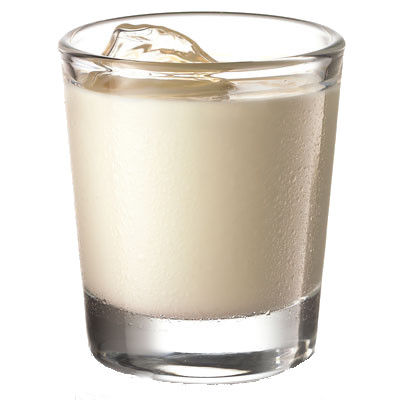
\includegraphics[width=5.5cm]{img/vasito.jpg}}
\tableofcontents\newpage

\section{Data structures}
\subsection{Segment tree}
\cppfile{data_structures/segment_tree.cpp}
\subsection{Segment tree - Lazy propagation}
\cppfile{data_structures/segment_tree_lazy.cpp}
\subsection{Segment tree - Persistence}
\cppfile{data_structures/segment_tree_persistent.cpp}
\subsection{Sparse table (static RMQ)}
\cppfile{data_structures/sparse_table.cpp}
\subsection{Fenwick tree}
\cppfile{data_structures/fenwick_tree.cpp}
\subsection{STL extended set}
\cppfile{data_structures/stl_extended_set.cpp}
\subsection{STL rope}
\cppfile{data_structures/stl_rope.cpp}
\subsection{Treap (implicit key)}
\cppfile{data_structures/treap_implicit.cpp}

\section{Graphs}
\subsection{Topological sort}
\cppfile{graphs/toposort.cpp}
\subsection{Kruskal (+ Union-Find)}
\cppfile{graphs/kruskal.cpp}
\subsection{Dijkstra}
\cppfile{graphs/dijkstra.cpp}
\subsection{Strongly connected components (+ 2-SAT)}
\cppfile{graphs/tarjan_2sat.cpp}
\subsection{Articulation - Bridges - Biconnected}
\cppfile{graphs/articulation_bridges_biconnected.cpp}
\subsection{LCA - Binary Lifting}
\cppfile{graphs/lca.cpp}
\subsection{Heavy-Light decomposition}
\cppfile{graphs/hld.cpp}

\section{Math}
\subsection{Integer floor division}
\cppfile{math/floor_division.cpp}
\subsection{Extended Euclid}
\cppfile{math/extended_euclid.cpp}
\subsection{Sieve of Eratosthenes}
\cppfile{math/sieve.cpp}
\subsection{Generate divisors}
\cppfile{math/divisors.cpp}
\subsection{Pollard's rho}
\cppfile{math/pollard_rho.cpp}

\section{Strings}
\subsection{Aho-Corasick}
\cppfile{strings/aho_corasick.cpp}
\subsection{Suffix automaton}
\cppfile{strings/suffix_automaton.cpp}

\section{Flow}
\subsection{Matching (slower)}
\cppfile{flow/matching.cpp}
\subsection{Hungarian}
\cppfile{flow/hungarian.cpp}
\subsection{Dinic}
\cppfile{flow/dinic.cpp}
\subsection{Min cost max flow}
\cppfile{flow/min_cost_max_flow.cpp}

\section{Other}
\subsection{Dates}
\cppfile{other/dates.cpp}

\end{document}
